\documentclass[10pt,letterpaper]{article}
% Official ICASSP 2027 Paper Kit style (downloaded 2026-09-22).
\usepackage{spconf}
% Keep the official geometry and typography; balance each text segment
% around anchored full-width displays instead of floating across paragraphs.
\onecolumn
\usepackage{multicol}
\usepackage{capt-of}
\setlength{\multicolsep}{6pt}
\raggedcolumns
\usepackage[hyphens]{url}
\usepackage{graphicx}
\usepackage{amsmath}
\usepackage{booktabs}
\usepackage{tabularx}
\usepackage{array}
\usepackage{tikz}
\usepackage{float}
\usetikzlibrary{arrows.meta,positioning}
\urlstyle{rm}
\def\UrlFont{\rm}
\usepackage{cite}
\frenchspacing
\raggedbottom
\widowpenalty=10000
\clubpenalty=10000

\pdfinfo{
/TemplateVersion (ICASSP 2027 official spconf)
}

\newcolumntype{Y}{>{\raggedright\arraybackslash}X}
\newcolumntype{L}[1]{>{\raggedright\arraybackslash}p{#1}}

\title{Are Self-Evolving Agent Skills Learning Skills?}
% Author names and affiliations must be supplied before non-blind submission.
\name{Anonymous Submission}
\address{}

\begin{document}
\ninept

\maketitle
\begin{multicols}{2}

\begin{abstract}

Self-evolving agents store experience in persistent skills, but a higher task score leaves open what useful behavior has become reusable. We diagnose completed SkillEvolver, SPARK, and CoEvoSkills artifacts through repeated paired evaluations and controlled task variations. Our analysis separates recurring aggregate utility from agreement on individual tasks, and decomposes the net gain into improvements and losses. We further distinguish gains on zero-reward tasks from interference with full-reward executions. All three methods improve source-task means in both runs, while task changes expose different scopes of utility. SkillEvolver sustains positive gains across the tested changes by combining more frequent improvements with fewer losses of existing success. These results characterize skill learning through the persistence and distribution of useful behavior beyond the source task.

\end{abstract}

\begin{keywords}
Agent skills, self-evolution, diagnostic evaluation, skill reuse, generalization
\end{keywords}

\section{Introduction}

Persistent agent skills offer a route to improvement without updating model parameters. Instructions, scripts, and supporting references make execution experience available to later runs. SkillEvolver, SPARK, and CoEvoSkills construct these artifacts through deployment-grounded revision, verified-trajectory distillation, and co-evolutionary verification~\cite{zhang2026skillevolver,zhou2026spark,zhang2026coevoskills}. Their outputs motivate the question in our title: when a system produces a higher-scoring skill, what useful behavior has become persistent?

The location of that improvement matters. A skill can preserve a decision rule that remains useful on new inputs, a choice tailored to the original instance, or a check that a later executor fails to apply. These artifacts may all help on the source task, yet lead to different outcomes when the task changes. The final score also combines artifact construction, execution, and verification. Understanding skill learning therefore requires following the stored guidance into the behavior it supports.

We ask two connected questions. \textbf{Does the benefit persist, and under which task changes?} Repeated source-task evaluations test whether paired utility recurs, while frozen-skill variants expose the demands that the same guidance can accommodate. \textbf{Which task-level changes produce the apparent improvement?} A positive mean may reflect widespread gains or a small balance between large benefits and losses. Identifying these patterns distinguishes the creation of useful behavior from interference with behavior the executor already performs successfully.

We examine three construction mechanisms through two standard-task runs per method and controlled changes to input representation, task instances, and coupled requirements. Each skill condition is paired with a no-skill execution of the same task. We then match task identities across runs, separate the positive and negative contributions to variant utility, and examine score transitions from the two baseline endpoints. The completed skill in use is the common object of diagnosis.

All three methods yield positive mean source-task gains in both runs, but this agreement does not persist under task variation. SkillEvolver remains positive across all three change types. SPARK's benefit depends on the change type, and CoEvoSkills has negative mean gains in all three. The clearest separation occurs when the instance is replaced. The decomposition explains how these means arise: all three methods produce substantial gains on some variants, while their frequency of improvement and cost to existing successes differ.

Our contribution is a diagnosis of the evidence behind observed skill gains. Repeated evaluations measure agreement across runs; controlled variants locate the scope of utility; gain--loss and baseline-conditioned analyses distinguish added benefits from disruption of existing success.

\section{Problem Formulation}

\subsection{Skill Revision and Evaluation}

At revision round $r$, an optimizer updates the current persistent skill artifact:
\begin{equation}
s_{r+1}=O(s_r,\tau_r,f_r),
\end{equation}
where $s_r$ is the current skill, $\tau_r$ is an execution trace, and $f_r$ is feedback from execution and evaluation. The operator $O$ denotes the method's complete update pathway, including its native merge, validation, selection, or adoption mechanism. A generated candidate that is rejected or never adopted is not $s_{r+1}$.

The agent then executes task $x$ with the frozen skill:
\begin{equation}
o_r=A(x,s_r,z_r),
\end{equation}
where $z_r$ represents model sampling, tool use, and environment state, and $o_r$ is the resulting output artifact or state change. A verifier maps the output to a score:
\begin{equation}
y_r=V(x,o_r).
\end{equation}

\end{multicols}
\noindent\begin{minipage}{\textwidth}
\centering
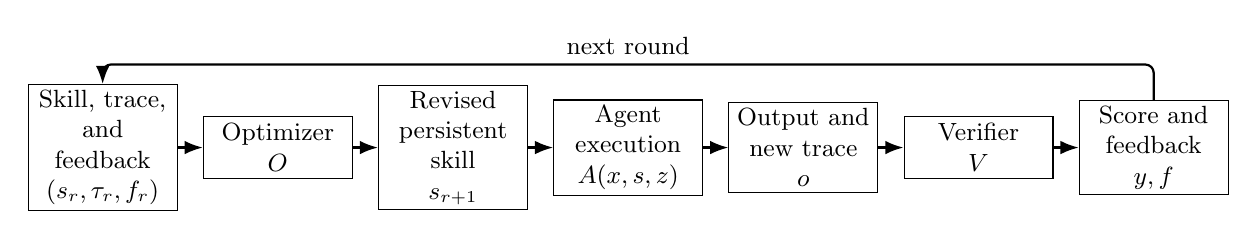
\begin{tikzpicture}[
  node distance=0.32cm,
  >=Latex,
  box/.style={draw, rectangle, align=center, minimum height=0.78cm, text width=1.75cm, inner sep=2pt, font=\small},
  arr/.style={->, thick}
]
\node[box] (evidence) {Skill, trace,\\and feedback\\$(s_r,\tau_r,f_r)$};
\node[box, right=of evidence] (optimizer) {Optimizer\\$O$};
\node[box, right=of optimizer] (skill) {Revised\\persistent skill\\$s_{r+1}$};
\node[box, right=of skill] (agent) {Agent execution\\$A(x,s,z)$};
\node[box, right=of agent] (output) {Output and\\new trace\\$o$};
\node[box, right=of output] (verifier) {Verifier\\$V$};
\node[box, right=of verifier] (score) {Score and\\feedback\\$y,f$};
\draw[arr] (evidence) -- (optimizer);
\draw[arr] (optimizer) -- (skill);
\draw[arr] (skill) -- (agent);
\draw[arr] (agent) -- (output);
\draw[arr] (output) -- (verifier);
\draw[arr] (verifier) -- (score);
\draw[arr, rounded corners=3pt] (score.north) -- ++(0,0.45) -| node[pos=0.25,above,font=\small]{next round} (evidence.north);
\end{tikzpicture}
\captionof{figure}{The skill-evolution lifecycle. Construction produces a persistent artifact; deployment turns its guidance into behavior; verification assigns the observed score. Our evaluation measures completed-artifact utility through paired outcomes, repeated runs, and frozen-skill task variation.}
\label{fig:lifecycle}
\end{minipage}
\par\vspace{6pt}
\begin{multicols}{2}

\subsection{From Score Gains to Skill Behavior}

The score $V(x,A(x,s,z))$ records the outcome of a skill used by an executor and assessed by a verifier. Comparing a completed skill with no skill measures its utility at deployment. Comparing the adopted final skill with its actual parent addresses the improvement associated with revision. The experiments here follow the first contrast across repeated runs and changed tasks.

For each source task $x$, we freeze its completed skill $s_x$ and evaluate it on a variant $T_k(x)$ alongside a no-skill execution. The skill remains unchanged, while the executor can reinterpret the input, recompute a solution, and adapt its actions. A positive paired difference on the variant indicates that the stored guidance remains useful under that change. The variation types distinguish the decisions that can be reused from those that the executor must reconsider.

To interpret the observed utility, we examine its distribution over tasks. Agreement between runs describes whether the same tasks benefit repeatedly. Separating positive and negative score changes reveals whether a small mean reflects small effects or cancellation. Conditioning on the no-skill score distinguishes help on zero-reward tasks from harm to full-reward executions. These measurements retain the paired task as the unit of analysis while answering different questions about the behavior associated with the skill.

\section{Does Skill Utility Persist beyond the Source Task?}
\label{sec:skillsbench-experiments}

We first test whether completed skills provide a recurring benefit on their source tasks. We then change the task while keeping its skill frozen to determine which demands that benefit survives. The paired no-skill execution provides the reference for both comparisons.

\subsection{Experimental Setup}

We evaluate SkillEvolver~\cite{zhang2026skillevolver}, SPARK~\cite{zhou2026spark}, and CoEvoSkills \cite{zhang2026coevoskills} on SkillsBench~\cite{li2026skillsbench}, with two runs per method. Each run pairs the method's skill condition with a no-skill execution of the same task. Both runs of each method use the same task set: 81 tasks for SkillEvolver, 84 for SPARK, and 85 for CoEvoSkills.

We report mean verifier reward on a 0--100 scale and the mean within-task difference between the skill and no-skill conditions. For a run with $N$ tasks, the paired gain is
\begin{equation}
\Delta = \frac{100}{N}\sum_{i=1}^{N}
\left(r_i^{\mathrm{skill}}-r_i^{\mathrm{no\text{-}skill}}\right).
\end{equation}
We also count tasks with positive, negative, and zero differences.

\subsection{Positive Source-Task Utility in Both Runs}

All three methods have positive mean paired gains in both runs (Table~\ref{tab:skillsbench-six-runs}). SkillEvolver gains 25.61 and 25.02 points, CoEvoSkills gains 10.24 and 9.76, and SPARK gains 1.84 and 6.45. SkillEvolver and CoEvoSkills retain similar gains despite substantial changes in their no-skill scores. The paired comparison reveals recurring utility that absolute skill-condition scores alone would obscure.

The task-level results also differ. SkillEvolver has at least four times as many improvements as regressions in each run; CoEvoSkills improves 17 tasks in each run, with nine and ten regressions. SPARK's first run is nearly balanced, while its second has 13 improvements and five regressions. The gain therefore reflects both the size and frequency of task-level changes. The frozen-skill variants test whether the useful guidance behind these source-task outcomes survives a different task demand.

\subsection{Do Evolved Skills Remain Useful When Tasks Change?}
\label{sec:variant-transfer}

A source-task skill may capture a reusable procedure, a decision rule, or assumptions specific to that instance. We deploy these skills on controlled variants while keeping each artifact frozen (Figure~\ref{fig:variant-evaluation}). The executor interprets the changed task and decides how to use the existing skill. Its reward difference from a no-skill execution of the same variant measures the final artifact's utility under that change.

\paragraph{Three forms of task change.}
Input-representation changes (P1) alter how the task is presented, including names, column arrangements, or schemas. They test whether the executor can recover the relevant roles of the inputs while using the skill. Task-instance changes (P2) replace the data or instance structure. They test whether the procedure can be instantiated with new values rather than relying on a solution specific to the source instance. Coupled-requirement changes (P3) alter or add requirements that must be handled together. They test whether the executor can adapt the procedure while preserving the constraints that determine a valid output. These changes probe different aspects of reuse rather than successive levels of difficulty.

The record contains 222 task variants and 886 condition-level results across no skill and the three methods. Table~\ref{tab:variant-transfer} summarizes historical and recovery evaluations for 222 SkillEvolver variants and 221 each for SPARK and CoEvoSkills. Panel B separates the within-variant differences by type of change.

\paragraph{Overall utility under task variation.}
SkillEvolver increases mean reward from 41.87 to 53.81, a gain of 11.94 points, with 47 improved and 20 regressed variants. Thus, its source-task skills retain positive average utility after the tasks change. SPARK increases mean reward from 41.61 to 42.25, a gain of 0.65 points, with 32 improvements and 37 regressions. The positive mean alongside more regressions than improvements reflects the magnitudes of the reward changes: the mean and the number of benefited variants capture different properties. CoEvoSkills decreases mean reward from 41.61 to 36.60, a change of $-5.01$ points, with 26 improvements and 41 regressions. Its positive source-task gains therefore coexist with negative average utility on the recorded variants.

\paragraph{Where does utility extend?}
SkillEvolver has positive gains under every type of change: 11.85 points on P1, 14.56 on P2, and 9.72 on P3. Improved variants also outnumber regressed variants within each type: 15 versus seven, 15 versus six, and 17 versus seven, respectively. Its overall gain consequently spans all three forms of variation. The largest mean gain occurs under P2, where applying the source skill requires working with a changed instance.

The other methods exhibit different profiles. SPARK remains positive on P1 and P3, at 2.00 and 4.53 points, but falls by 5.23 points on P2. CoEvoSkills has negative average changes on all three types, with its largest decline also on P2 ($-9.51$ points, compared with $-3.59$ on P1 and $-2.42$ on P3). Instance changes thus separate the observed reuse profiles especially clearly: SkillEvolver's largest positive gain and the other methods' largest declines occur in the same category of variation.

\paragraph{What the combined results reveal.}
All three methods obtain positive mean gains in both standard-task runs, yet their variant profiles differ substantially. Success on the source tasks and usefulness after task changes are distinct empirical properties. SkillEvolver provides the clearest positive reuse pattern in these records, whereas SPARK's benefit depends on the type of change and CoEvoSkills' source-task benefit does not extend on average. Approximately seven in ten variants remain tied with the baseline for each method. The gains therefore arise from a subset of changed outcomes, motivating a closer examination of the decisions expressed when a skill helps or hinders execution.

\begin{figure*}[t]
\centering
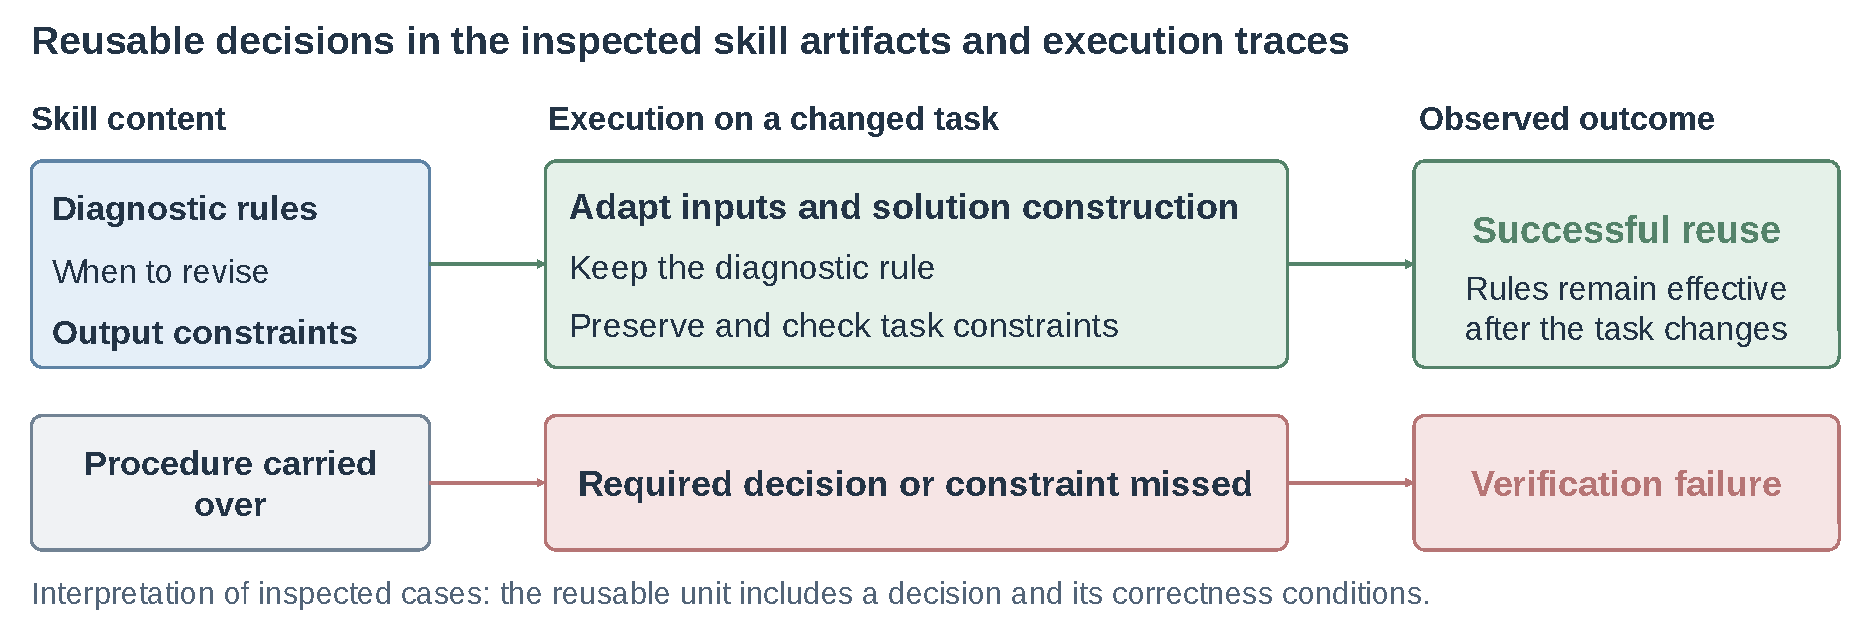
\includegraphics[width=\textwidth]{figures/skill-reuse-logic.pdf}
\caption{Skill reuse in the inspected cases. Diagnostic rules guide adaptation, and correctness constraints guide output checks. Successful reuse preserves these decisions while adapting the solution; unsuccessful reuse can carry over a procedure while missing a required decision or constraint.}
\label{fig:skill-reuse}
\end{figure*}

\subsection{What Is Preserved When a Skill Is Reused?}
\label{sec:skill-reuse}

To interpret the variant results, we inspect the skill artifacts together with their execution traces. We distinguish the procedure stored in a skill from the way an executor applies it to a new task. A script can preserve an action sequence, while successful reuse also depends on recognizing when that sequence applies, adjusting its inputs, and checking its output. Figure~\ref{fig:skill-reuse} organizes the inspected evidence around these decisions.

\paragraph{Diagnostic rules guide adaptation.}
In the inspected SkillEvolver artifacts, intermediate checks guide the choice and revision of a procedure. Candidate discovery, diagnosis, and refinement appear as separate operations, with conditions explaining when to revisit an intermediate result. This structure gives the executor opportunities to respond to changed inputs before committing to an output. In the signal-detection traces, for example, the executor uses diagnostic checks to distinguish competing candidate explanations and adjusts the search accordingly. The reusable content is the rule for evaluating a candidate; the candidate values and search settings can change with the task.

\paragraph{Correctness constraints survive solution changes.}
A second form of reusable content specifies which properties the output must preserve. The inspected scheduling skill expresses constraints relative to the supplied instance and baseline, allowing the executor to construct a different schedule while checking the same repair requirements. Failure traces make this distinction visible: much of a workflow can execute correctly while one omitted requirement invalidates the final result. This helps explain why preserving a familiar procedure is insufficient when a variant changes how inputs are represented or how requirements interact.

\paragraph{Reuse combines preserved rules with new execution.}
Across the inspected cases, successful adaptation preserves decision criteria and correctness checks while changing input handling, search choices, or the constructed solution. This illustrates how a transferred artifact can help the executor decide what to retain and what to recompute. SkillEvolver's positive profile across P1--P3 is consistent with this form of reuse. The trace evidence identifies concrete instances of that behavior. Complementary interventions on SkillRevise, SkillHone, and SkillOpt later in the paper test component effects within their respective artifact lineages.

The variant evaluations characterize how far final-skill utility extends beyond the source task. The following retention and lifecycle studies examine whether improvements persist under fresh deployment and which parts of the evolution process produce them.



\section{Analysis}
\label{sec:analysis}

We distinguish three contributors to mean utility: agreement on which tasks improve across runs, the balance between positive and negative changes, and whether the skill helps or harms execution at different no-skill reward levels.

\subsection{Recurring Means Do Not Imply the Same Tasks Improve}

Matching task identities across the two source-task runs reveals how much of the positive mean comes from recurring improvements. SkillEvolver improves 27 tasks in run 1 and 26 in run 2, but only 14 improve in both. The corresponding overlaps are three for SPARK and seven for CoEvoSkills. Across tasks that improve at least once, these counts are 14 of 39, three of 19, and seven of 27. Thus, the nearly unchanged mean gains of SkillEvolver and CoEvoSkills coexist with changes in which tasks benefit.

The transitions clarify this variation. Of SkillEvolver's 27 first-run improvements, 14 remain improvements, 12 become ties, and one becomes a regression. SPARK's nine first-run improvements become three improvements, four ties, and two regressions. CoEvoSkills' 17 become seven improvements, nine ties, and one regression. Losing an observed advantage most often means becoming tied with the no-skill execution, rather than reversing the sign. Conversely, ten, seven, and ten tasks move from a first-run tie to a second-run improvement for SkillEvolver, SPARK, and CoEvoSkills, respectively.

CoEvoSkills also regresses on five of the same tasks in both runs; neither other method has a task that regresses twice. This identifies a recurring source-task cost within a positive overall mean. The two runs therefore supply two distinct observations: each method has positive aggregate utility twice, while the task identities supporting that utility are only partly shared. These are comparisons of paired outcomes across runs; the shared object is the task, with each run using its recorded skill condition and execution.

\subsection{Benefits and Losses Can Nearly Cancel}

To distinguish small effects from cancellation, let $d_i=r_i^{\mathrm{skill}}-r_i^{\mathrm{no\text{-}skill}}$. We separate the variant mean into positive and negative contributions:
\begin{equation}
G=\frac{100}{N}\sum_i\max(d_i,0),\quad
L=\frac{100}{N}\sum_i\max(-d_i,0).
\end{equation}
The paired gain is $\Delta=G-L$. Both terms use all evaluated variants as their denominator, so they account for the frequency and magnitude of score changes together.

SkillEvolver contributes 18.89 points of improvement against 6.95 points of loss, leaving the observed $+11.94$ gain. SPARK contributes 13.73 positive points and 13.08 negative points. Its $+0.65$ mean therefore masks substantial movement in both directions. CoEvoSkills contributes 10.98 positive points, but its 15.98-point loss outweighs them. Its negative average includes useful changes on some variants alongside a larger cost elsewhere.

The conditional magnitudes further distinguish these patterns. Among improved variants, the average increase is 89.23 points for SkillEvolver, 94.82 for SPARK, and 93.30 for CoEvoSkills. Among regressed variants, the average loss is 77.16, 78.15, and 86.16 points. All three methods can produce large gains where they help. Their overall separation comes from how often those gains occur and how much is lost on other variants, rather than SkillEvolver alone producing large individual improvements. Its 47 improvements and 20 regressions give positive changes more weight; the balance reverses for SPARK (32 versus 37) and CoEvoSkills (26 versus 41).

\subsection{Helping Zero-Reward Tasks and Preserving Full-Reward Tasks}

Conditioning on the no-skill reward gives the changes a concrete interpretation. Each method's variant set contains 126 zero-reward no-skill executions. SkillEvolver raises 42 of them to positive reward, including 40 to full reward. SPARK raises 30 to full reward, and CoEvoSkills raises 25 to positive reward, including 23 to full reward. The respective rates of moving beyond zero are 33.3\%, 23.8\%, and 19.8\%. SkillEvolver's advantage thus includes more frequent gains on variants where the executor receives no verifier credit without the skill.

The other endpoint measures losses on variants with a full-reward no-skill execution. Among SkillEvolver's 86 full-reward no-skill variants, 16 fall below full reward, including 15 that fall to zero. SPARK lowers 29 of 85, including 27 to zero; CoEvoSkills lowers 32 of 85, all to zero. The rates of losing full reward are 18.6\%, 34.1\%, and 37.6\%. Each method also has ten intermediate-baseline variants, which remain included in the aggregate results but are outside these endpoint counts.

These two directions explain why counting newly successful tasks alone is insufficient. SPARK and CoEvoSkills both turn many zero-reward cases into full-reward outcomes, yet lose full reward on almost as many or more baseline successes. SkillEvolver combines the highest rate of gains from zero with the lowest rate of losses from full reward. Its broader utility is expressed in both acquiring a benefit and preserving outcomes that the executor already achieves.

\subsection{Useful Guidance Must Survive a Change in Demand}

Source-task utility establishes whether a completed skill helps on the task from which it was constructed. Frozen-skill variants test whether its guidance remains useful when original details no longer apply. Their three demands---remapping inputs, recomputing instance-dependent choices, and accommodating coupled requirements---probe different scopes of useful behavior.

This distinction is central to the observed method profiles. SPARK retains positive means under P1 and P3 but becomes negative under P2. Its source-task benefit therefore does not extend uniformly to replacement instances. CoEvoSkills has positive source-task means but negative means under every variant type. SkillEvolver combines positive means with more improvements than regressions in each type. The latter profile is the broadest evidence of useful generalization in these evaluations: the frozen guidance remains beneficial across different demands on the executor.

The published construction procedures suggest where these demands enter skill learning. SkillEvolver contrasts successful and failed deployments and audits reliance on training-instance constants~\cite{zhang2026skillevolver}; SPARK distills environment-verified execution trajectories~\cite{zhou2026spark}; CoEvoSkills uses a co-evolving surrogate verifier to supply detailed revision feedback~\cite{zhang2026coevoskills}. These mechanisms draw on different evidence when retaining guidance. Our behavioral results make abstraction from the source instance a concrete target for explaining their differences, especially the divergence under P2. Testing that explanation would require changing the construction feedback while holding the evaluation fixed.

\subsection{Learning a Useful Skill Includes Avoiding Interference}

The endpoint analysis adds a second requirement to generalization: a skill should help when the executor struggles without displacing decisions it already makes correctly. The no-skill condition makes both directions observable. Moving from zero to positive reward indicates additional useful behavior in the recorded execution. Falling from full reward identifies a lower-scoring skill execution paired with a full-reward no-skill execution. Reporting only the former would conceal a substantial part of the effect.

The SPARK and CoEvoSkills results show why this distinction changes the interpretation of learning. Both produce many large improvements, so their weak or negative variant means cannot be explained by an absence of helpful skills. Instead, their gains are offset by losses elsewhere. SkillEvolver's stronger net utility combines more gains from zero with fewer disruptions of full-reward outcomes. The diagnostic target is therefore the distribution of useful guidance: where it adds value, where it remains unnecessary, and where it interferes with execution.


\section{Interpreting Gains as Evidence of Skill Learning}

\subsection{Useful Guidance Must Survive a Change in Demand}

Source-task utility establishes whether a completed skill helps on the task from which it was constructed. Frozen-skill variants test whether its guidance remains useful when original details no longer apply. Their three demands---remapping inputs, recomputing instance-dependent choices, and accommodating coupled requirements---probe different scopes of useful behavior.

This distinction is central to the observed method profiles. SPARK retains positive means under P1 and P3 but becomes negative under P2. Its source-task benefit therefore does not extend uniformly to replacement instances. CoEvoSkills has positive source-task means but negative means under every variant type. SkillEvolver combines positive means with more improvements than regressions in each type. The latter profile is the broadest evidence of useful generalization in these evaluations: the frozen guidance remains beneficial across different demands on the executor.

The published construction procedures suggest where these demands enter skill learning. SkillEvolver contrasts successful and failed deployments and audits reliance on training-instance constants~\cite{zhang2026skillevolver}; SPARK distills environment-verified execution trajectories~\cite{zhou2026spark}; CoEvoSkills uses a co-evolving surrogate verifier to supply detailed revision feedback~\cite{zhang2026coevoskills}. These mechanisms draw on different evidence when retaining guidance. Our behavioral results make abstraction from the source instance a concrete target for explaining their differences, especially the divergence under P2. Testing that explanation would require changing the construction feedback while holding the evaluation fixed.

\subsection{Learning a Useful Skill Includes Avoiding Interference}

The endpoint analysis adds a second requirement to generalization: a skill should help when the executor struggles without displacing decisions it already makes correctly. The no-skill condition makes both directions observable. Moving from zero to positive reward indicates additional useful behavior in the recorded execution. Falling from full reward identifies a lower-scoring skill execution paired with a full-reward no-skill execution. Reporting only the former would conceal a substantial part of the effect.

The SPARK and CoEvoSkills results show why this distinction changes the interpretation of learning. Both produce many large improvements, so their weak or negative variant means cannot be explained by an absence of helpful skills. Instead, their gains are offset by losses elsewhere. SkillEvolver's stronger net utility combines more gains from zero with fewer disruptions of full-reward outcomes. The diagnostic target is therefore the distribution of useful guidance: where it adds value, where it remains unnecessary, and where it interferes with execution.

\section{Related Work}

\noindent\textbf{Learning persistent skills from experience.}
SkillEvolver, SPARK, and CoEvoSkills make experience persistent through different construction loops: deployment-grounded revision, verified-trajectory distillation, and co-evolutionary verification, respectively~\cite{zhang2026skillevolver,zhou2026spark,zhang2026coevoskills}. These methods motivate our focus on the artifact delivered to a later executor. We study how that artifact's usefulness changes after its source task is varied, and analyze the task-level benefits and losses that produce its overall utility.

\noindent\textbf{Evaluating skill utility and use.}
SkillsBench evaluates skill utility across diverse tasks, while SWE-Skills-Bench studies skill use in software engineering~\cite{li2026skillsbench,han2026sweskillsbench}. SkillLearnBench evaluates continual skill generation on real-world tasks~\cite{zhong2026skilllearnbench}. From Raw Experience to Skill Consumption separates experience generation, skill extraction, and downstream consumption~\cite{huang2026rawexperience}. Our study connects these evaluation levels to the identification of skill learning: repeated outcomes characterize completed-skill utility, task changes test its persistence, and score-transition analyses distinguish added benefits from losses of existing success. The unit of interpretation is the persistent artifact in use.

\section{Conclusion}

Our diagnosis examines what score gains from self-evolving skills represent beyond the source task. All three methods improve source-task means in two runs, but the individual tasks benefiting from them only partly recur. Frozen-skill variants expose different scopes of generalization, with SkillEvolver sustaining positive utility across representation, instance, and requirement changes. Decomposing the results shows that all three methods can deliver large individual gains; their net utility depends on the frequency of those gains and the losses incurred elsewhere. SkillEvolver combines more frequent gains from zero reward with fewer disruptions of full-reward executions. These findings connect the learning question to observable behavior: reusable guidance should add useful capability, retain its value when the task changes, and preserve success that the executor already achieves.

\end{multicols}
\clearpage
\begin{multicols}{2}
{\small
\bibliographystyle{IEEEbib}
\bibliography{references}
}

\end{multicols}
\end{document}
